\documentclass[12pt]{article}
\usepackage[a4paper, margin=2cm]{geometry}
\setlength{\parindent}{0pt}
\usepackage{graphicx}
\graphicspath{ {../images/} }
% Title information
\title{Réseaux : notes de cours}
\author{Arian Dervishaj}
\date{\today}

\begin{document}
\maketitle
\pagebreak

\subsection*{Topologie réseau}
\begin{minipage}{0.3\textwidth}
    \begin{itemize}
        \item Point à point
        \item Bus
        \item Ring
        \item Star
        \item Full mesh
        \item Étoile étendue
        \item Distribué
    \end{itemize}
\end{minipage}
\begin{minipage}{0.6\textwidth}
    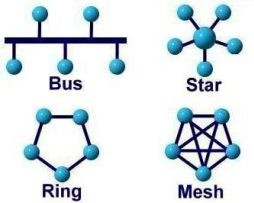
\includegraphics{topologie.jpeg}
\end{minipage}

\subsection*{Exigence 1 : Connectivité (p.19)}


\textbf{Point à point (full mesh) }: \# noeuds = $\frac{m(m-1)}{2}$ (gros problème en coût)\\
\textbf{Bus} : \# noeuds = $1+m$

\subsubsection*{Lexiques des composants réseaux}
\begin{enumerate}
    \item Applicaiton : Utilise le réseau (Skype, ...)
    \item Hôte : Supports apps (Laptop, ...)
    \item Routeur : Relaie des messages entre des liens (Access point, ...)
    \item Lien, canal : Connecte les noeuds (Wireless, wires, ...)
\end{enumerate}

\subsubsection*{Valeur d'un réseau}
La valeur d'un réseau de N noeuds est proportionnelle à $N^{2}$. \\
Grand réseau + de valeur qu'un petit réseau.

\subsection*{Exigence 2 : Partage des ressources efficace (p.26-27)} 


\textbf{Multiplexage (temporel, synchrone)} : chaque interval de temps $->$ nouveau slot alloué meme si pas utilisé. 
Capacité d'accès au réseau est limité au nombre de slot.

\textbf{Multiplexage statistique} : Les données sont stocké dans l'equipement et en fonction de la capacité de calcul de l'équipement, envoie les données.
Dépend de la capacité de l'équipement.


\subsection*{Exigence 3 : Abstraction commune aux applications (p.28-30)}


Chaque app doit avoir une couche d'abstraction commune pour communiquer (\textbf{les sockets}).

\subsubsection*{Modèles de communication courants}
\begin{enumerate}
    \item   Client - Serveur (topologie en étoile). \\
            $-$ : Quasi toutes les apps sont implémentés comme ça.
            Si le serveur tombe, tout tombe. Soucis de confidentialitée. \\
            + : Facile à gérer.
    \item   Pair à Pair \\
            Chaque machine est client et serveur. \\
            $+$ : Plus résilient. \\
            $-$ : Faut découvrir les autres du réseaux. Les données sont éphémères.
\end{enumerate}

\subsubsection*{Fiabilité}

Internet est un réseau "best effort". Un noeud peut tombé en panne n'importe quand.

\subsection*{Exigence 4 : (inter) opérabilité (p.31)}
Impact majeur sur le déploiment des réseaux aujourd'hui.

Comment on fait face : 
\begin{itemize}
    \item On ne change rien
    \item On structure
    \item On automatise
    \item On standardise
\end{itemize}

\subsection*{Architecture de réseau (p.33-34)}

Plus la couche est haute, plus il y'a de changement car moins de contraintes.

\subsection*{Protocoles}
\dots

\subsection*{Couches de réseaux}

\textbf{Modele OSI (théorique)}
\begin{itemize}
    \item couche phyisique : Gère la transmission (analogique $->$ binaire).
    \item Couche de liaison : Collecte un flux, framing.
    \item Couche réseau : Gère le routage.
    \item Couche transport : Envoie l'info de bout en bout. Pallie aux erreur (renvoie les paquets perdus, checksum)
    \item Couche Session : Fournit un espace de noms pour relier les flux
    \item Couche de présentation : Préoccupé par le format des données
    \item Couche d'application : Normaliser le type commun d'échanges (HTTP, \dots)
\end{itemize}

\textbf{Architecture Internet (modèle TCP/IP)}
\begin{itemize}
    \item Applicaiton
    \item TCP / UDP
    \item IP
    \item Subnetwork
\end{itemize}

\begin{minipage}{0.6\textwidth}
    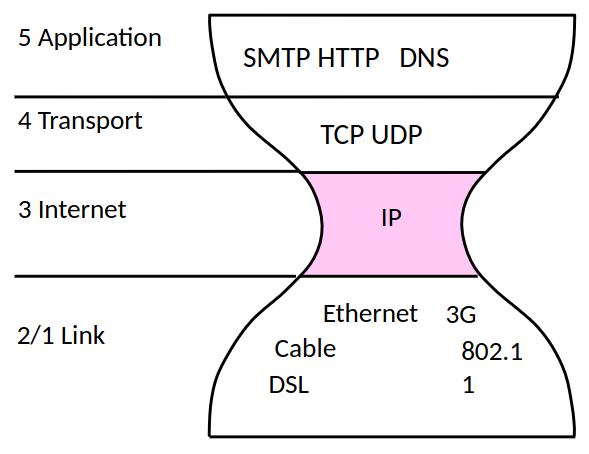
\includegraphics[scale=0.4]{architecture_internet_sablier.png}
\end{minipage}
\end{document}